\chapter{RESULTADOS PRELIMINARES}

Los resultados preliminares se han desarrollado con el fin de cumplir con el primer objetivo secundario, diseñar e implementar algoritmos de visión computacional y aprendizaje automático capaces de reconocer y cuantificar agujeros de red y nivel de suciedad. Como fue presentado en el capítulo \ref{MARCO_METODOLOGICO} en el inciso \ref{VIP_SLAM}, se simulará SLAM visual-inercial-presión con 3 etapas. Para la primera, uso de SLAM visual monocular con ORB-SLAM2.

Dentro del simulador Gazebo se utilizó un Turtlebot3, la cámara de un Kinect y un sensor IMU. A este último sensor se agregó un filtro de Kalman extendido para reducción de error de medición. Asimismo se realizó una malla de 1.75 m por 1 m de diámetro como se muestra en la figura \ref{fig:malla}.

\begin{figure} [!h]
    \begin{center}
    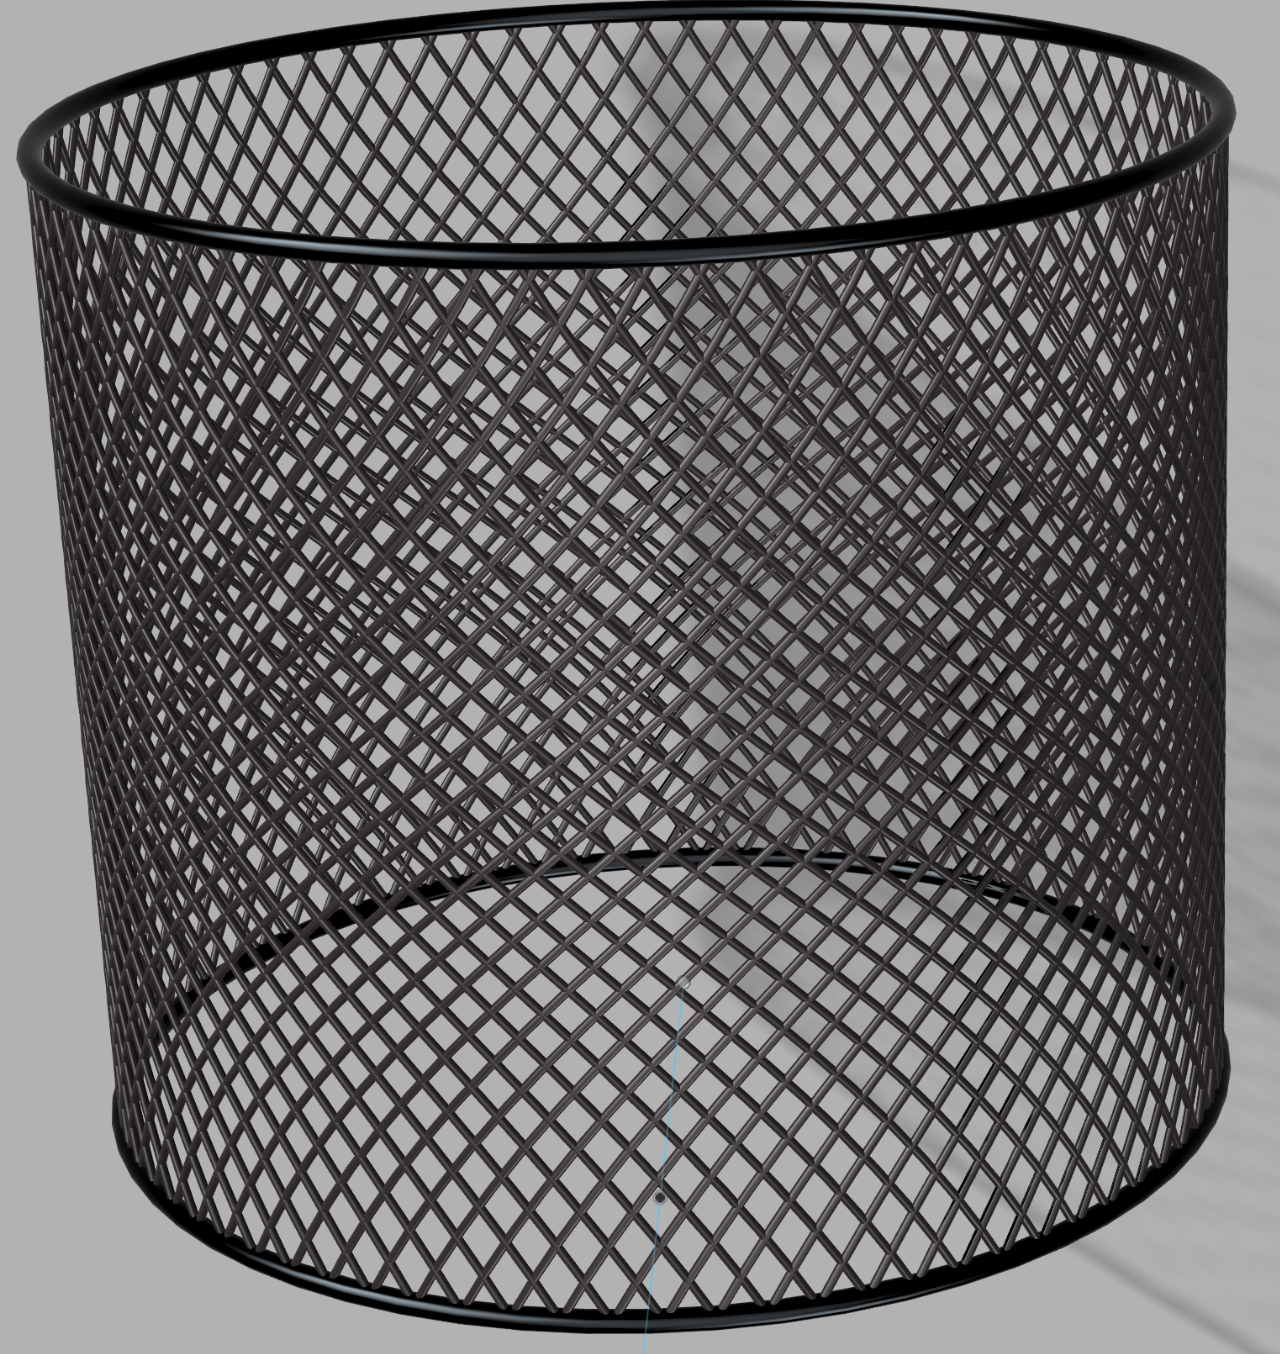
\includegraphics[height=6cm]{images/malla} 
    \caption{\label{fig:malla}Elaboración propia de una malla.}
    \end{center}
\end{figure}

Una vez el algoritmo esté corriendo, se obtuvo el diagrama de tópicos y nodos mostrados en la figura \ref{fig:rqt_graph}. Se puede apreciar que el algoritmo como nodo 'orb\_slam2\_mono' usa información del sensor IMU con filtro Kalman extendido 'nodo\_imu\_ekf' publicado en el tópico 'tf'. Del mismo modo, utiliza las imágenes publicadas en el tópico 'image\_raw' del Kinect. 

\begin{figure}[!h]
    \begin{center}
    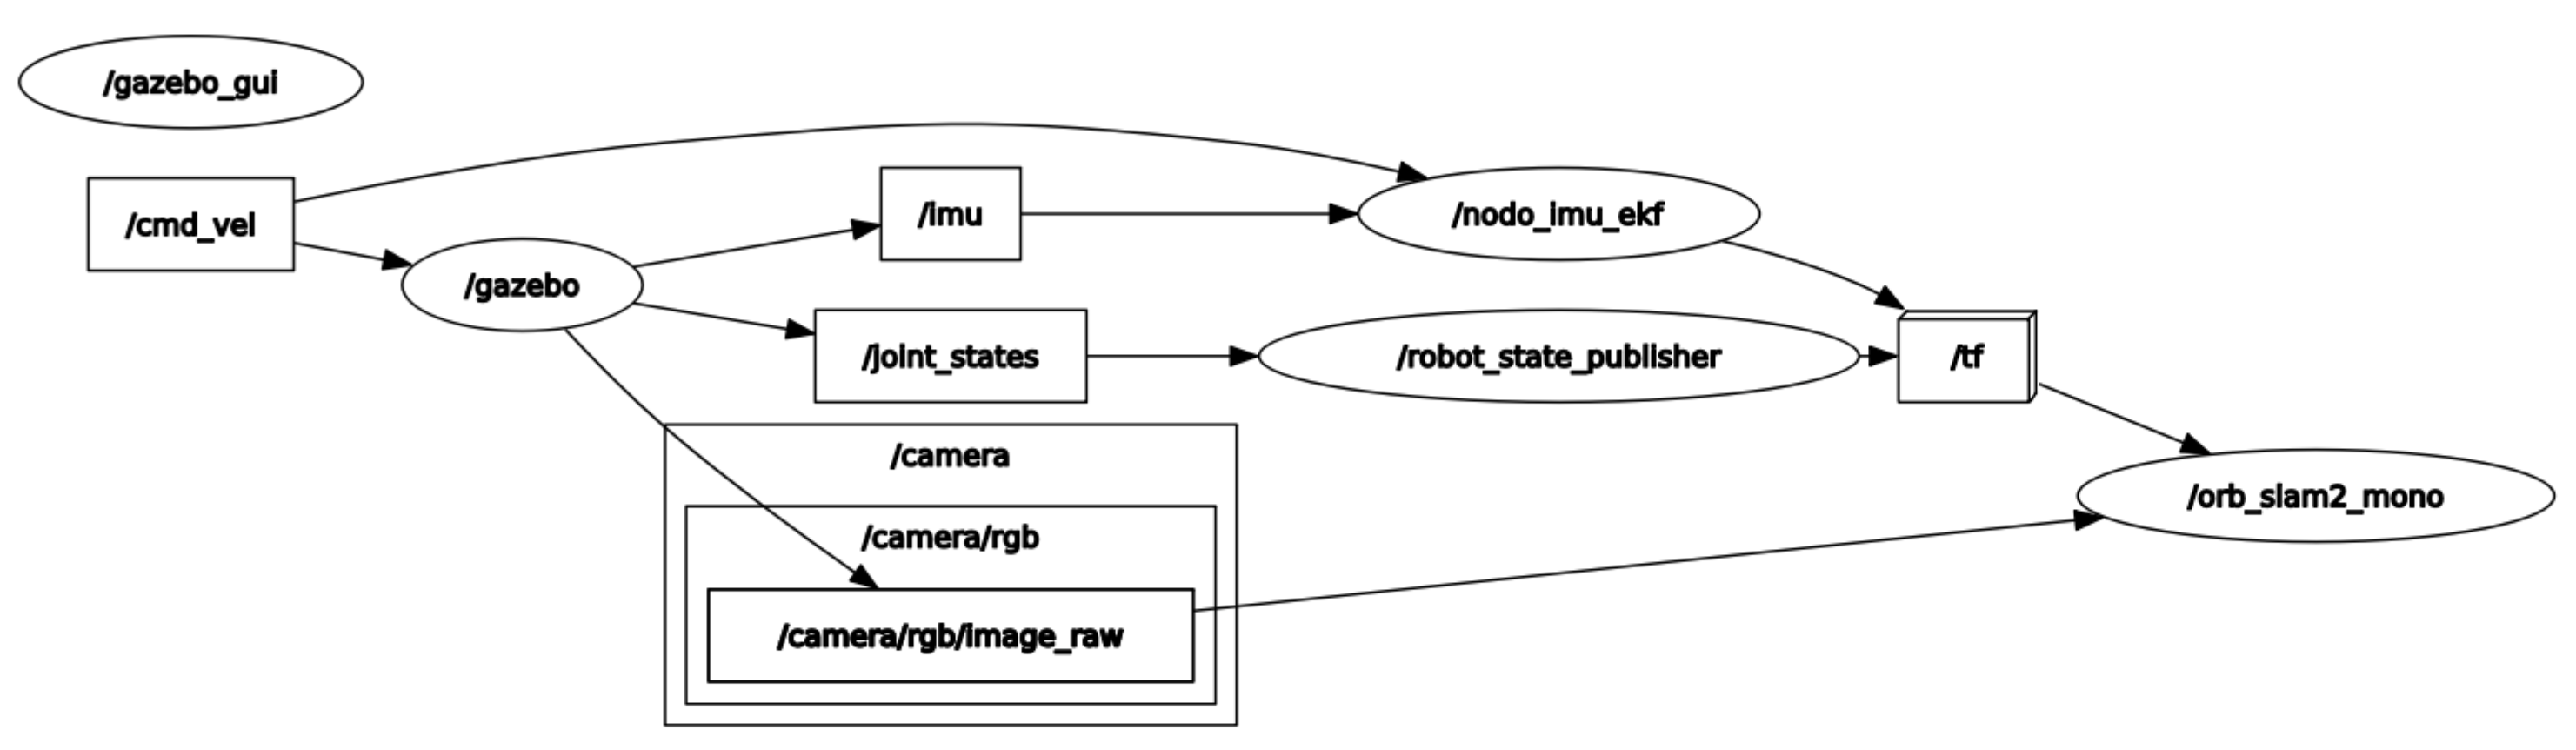
\includegraphics[height=4cm]{images/rqt_graph} 
    \caption{\label{fig:rqt_graph}Diagrama de tópicos y nodos en ROS.}
    \end{center}
\end{figure}

En la figura \ref{fig:sim_ros} se aprecia el entorno en Gazebo en (a), donde la luz tiene un tono azulado. En (b) en ell visualizador RViz se tiene el turtlebot moviendo, donde ya encuentra los keypoints de la red. 

\begin{figure} [!h]
    \begin{center}
    \begin{tabular}{cc}
    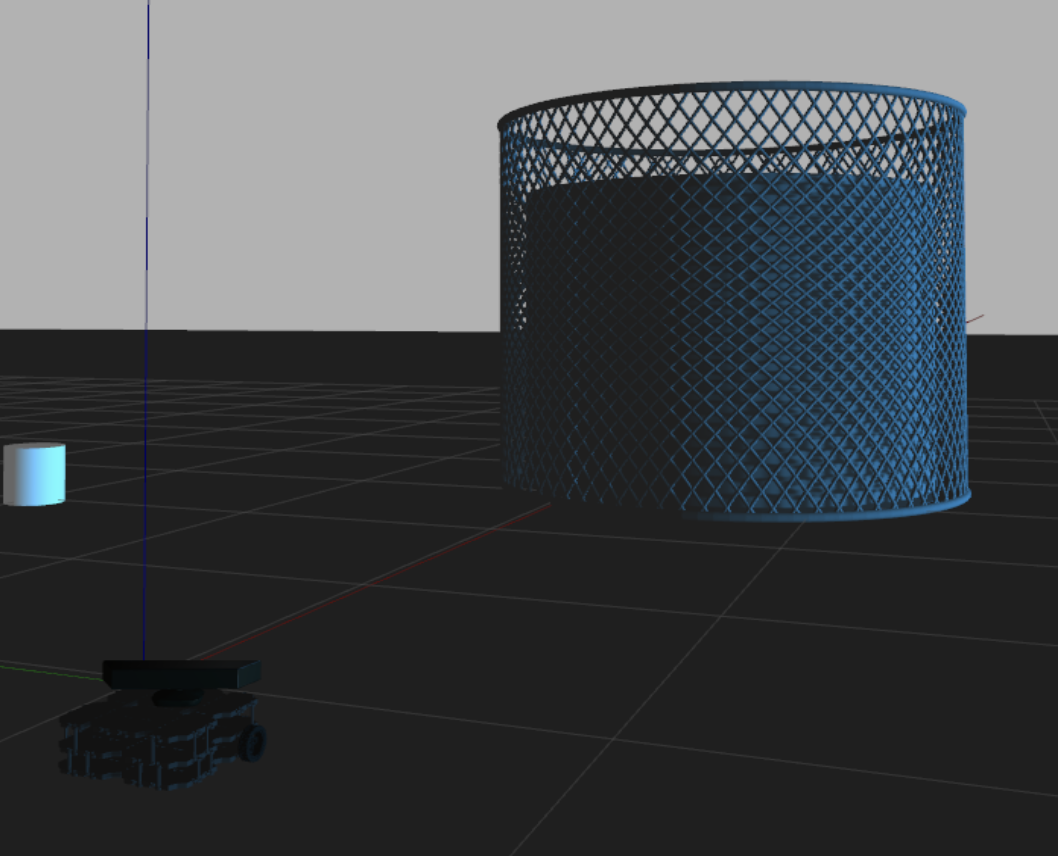
\includegraphics[height=5cm]{images/gazebo_1}
    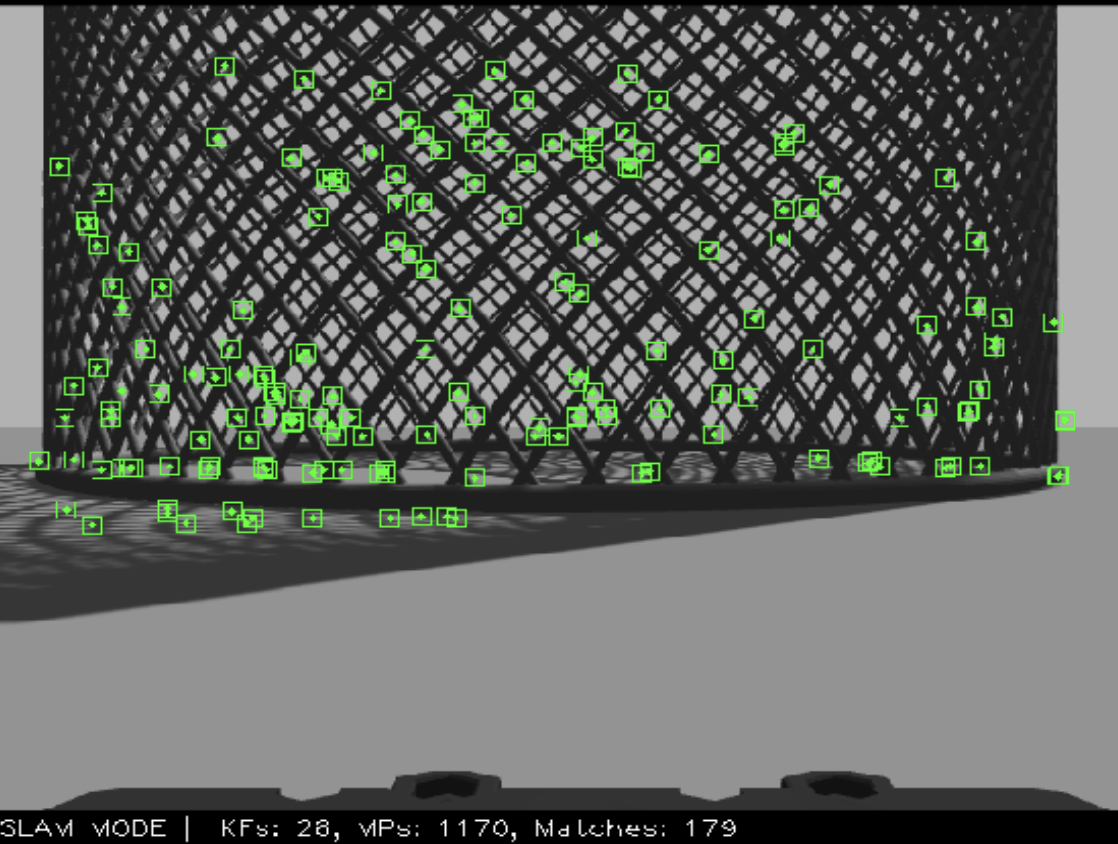
\includegraphics[height=5cm]{images/rviz_1} \\
    (a) & (b)
    \end{tabular}
    \caption{\label{fig:sim_ros}Turtlebot en (a) Gazebo y (b) RViz en la búsqueda de keypoints.}
    \end{center}
\end{figure}

La reconstrucción en RViz se puede apreciar en la figura \ref{fig:sim_ros_1}. En (a) se puede apreciar la reconstrucción a partir de las imágenes captadas, mientras que en (b), los keypoints encontrados. En el primero se resalta que el robot no logra encontrar los keypoints de la parte posterior, y se asume que es por la confusión de los keypoints encontrados en la parte trasera de la malla respecto a dónde se encuentra. Asimismo, al intentar construir la parte trasera del robot se puede apreciar unas líneas faltantes, siendo estas la red de la parte posterior de la malla.

\begin{figure} [!h]
    \begin{center}
    \begin{tabular}{cc}
    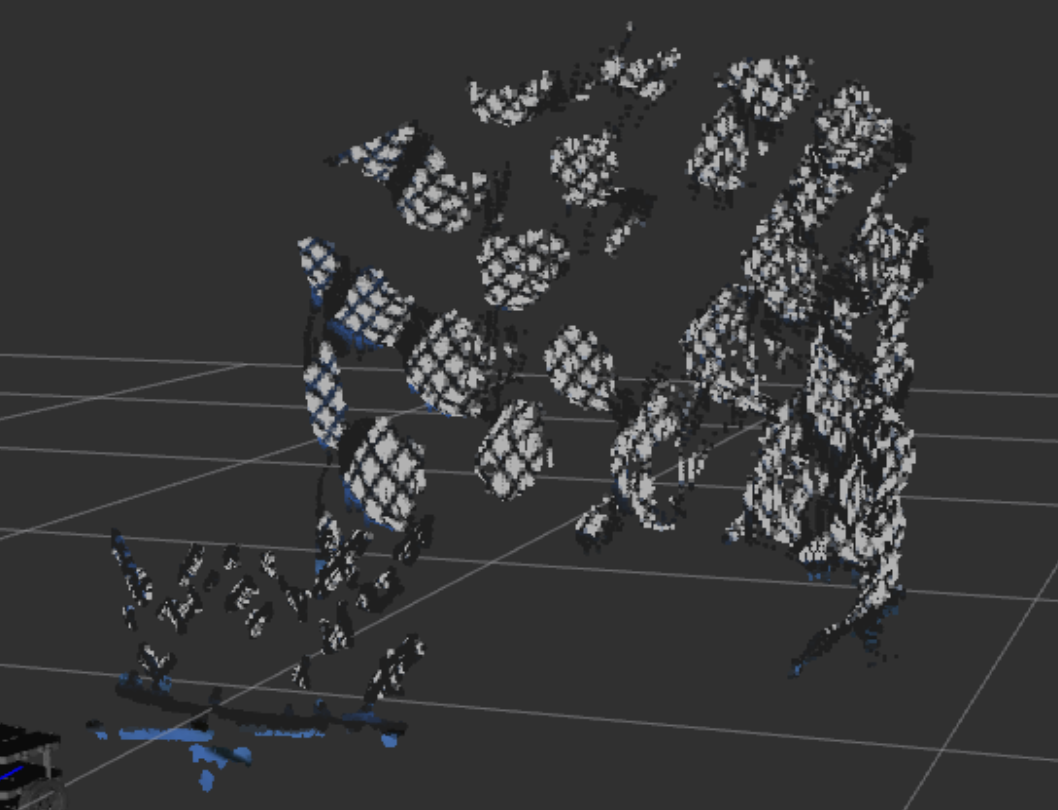
\includegraphics[height=5cm]{images/rviz_2}
    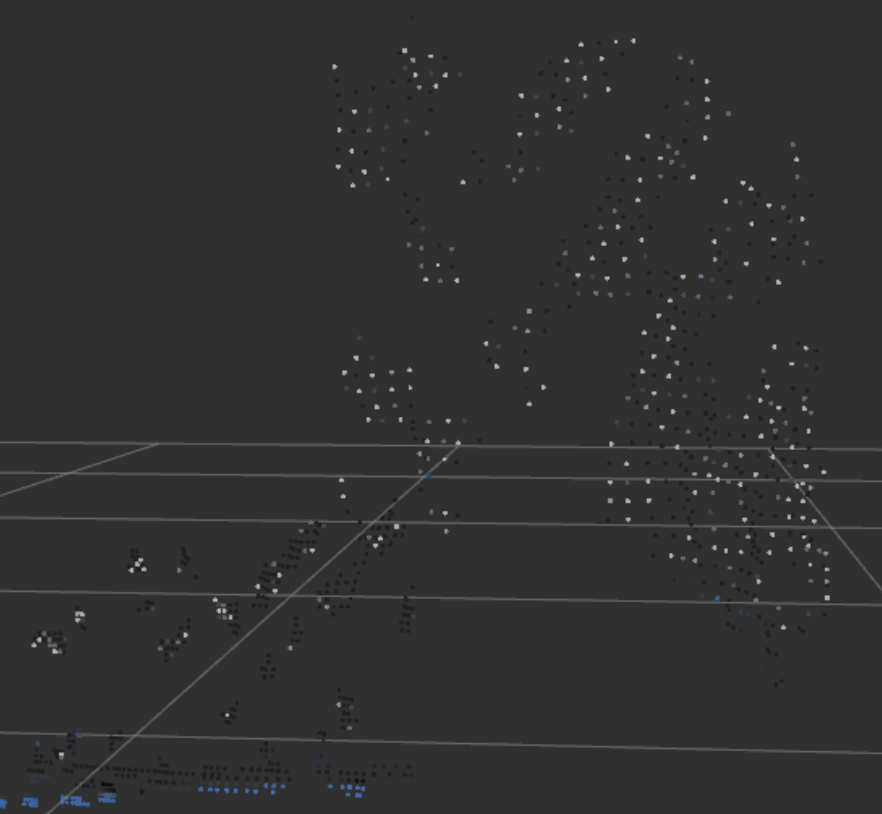
\includegraphics[height=5cm]{images/rviz_3} \\
    (a) & (b)
    \end{tabular}
    \caption{\label{fig:sim_ros_1}Reconstrucción en RViz en (a) a partir de las imágenes, y en (b) a partir de los keypoints.}
    \end{center}
\end{figure}

Estos resultados se pueden alejar de la realidad, ya que la parte trasera de la red no se aprecia bajo el mar debido a la turbidez del agua, por lo que se propone para siguientes pruebas este cambio. Por otro lado, el Turtlebot, al no tener un grado de libertad en el eje z, no se puede elevar. Por ese lado, se buscará un robot como un dron u otro simulador capaz de utilizar otro robot robot con este grado de libertad.
